\section{Theorie}
\label{sec:Theorie}

Magnetfelder werden induziert, wenn sich elektrische Ladungen bewegen. Die magnetische Feldstärke $\vec{H}$ beschreibt ihre Richtung und ihren Betrag.
Eine weitere Größe, welche Magnetfelder beschreibt, ist die magnetische Flußdichte $\vec{B}$. Ein Zusammenhang dieser beiden vektoriellen Größen besteht über die Permeabilität $\mu$:
\begin{equation*}
    \vec{B} = \mu_0 \mu_r \cdot \vec{H} ,
\end{equation*}
wobei $\mu_0 = 4\pi \cdot 10^-7$ die Vakuum-Permeabilität ist und $\mu_r$ die relative Permeabilität.
Wird ein stromdurchflossener Leiter, wie zum Beispiel ein Draht, von einem Magnetfeld umgeben, kann man das Magnetfeld berechnen mit dem Biot-Savartschen Gesetz
\begin{equation*}
    d\vec{B} =  \frac{\mu_\text{0}I}{4\pi}\,\frac{d\vec{s}\times\vec{r}}{r^3} .
\end{equation*}
Zur Berechnung des Manetfeldes innerhalb einer langen stromdurchflossenen Spule, dient die Formel
\begin{equation}
   B = \mu_0 \mu_r \frac{n}{l} I ,
\end{equation}
mit Spulenlänge $l$, Windungszahl $n$ und Spulenstrom $I$.
Das Feld einer solchen Spule ist in der Mitte homogen und außerhalb inhomogen.
Das Magnetfeld außerhalb einer Ringspule mit Radius $r_T$ ist außerhalb Null. Innerhalb lässt sich das homogene Magnetfeld durch
\begin{equation}
   B = \mu_0 \mu_r \frac{n}{2\pi r_T} I 
\end{equation}
bestimmen.

\noindent Um ein homogenes Magnetfeld zu erzeugen, wird ein Helmholtzspulenpaar genutzt, wie in Abbildung (1) zu sehen is.
Das Magnetfeld in der Mitte dieser Spulen mit Radius $R$ und einer Windung ergibt sich zu
\begin{equation}
   B(0) = \frac{\mu_\text{0}IR^2}{(R^2+x^2)^{3/2}} .
\end{equation}
Dabei ist x der Abstand zum Mittelpunkt.
\begin{figure}[H]
  \centering
  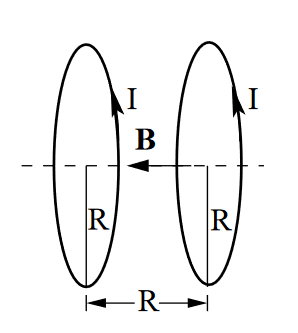
\includegraphics[height=5cm]{Screenshot (2)}
  \caption{Anordnung der Helmholtz-Spulen. \cite[S. 2]{sample}}
\end{figure}

\noindent Eine Form von Magnetismus in Materialien ist der Ferromagnetismus. Diese Materialen besitzen ohne äußeres Magnetfeld ein permanentes magnetisches Moment. 
Diese richten sich in Weiß'schen Bezirken parallel zueinander aus.
Für ferromagnetische Materialien beschreibt die Hysteresekurve (Abbilgun (2)) den Verlauf des Magnetfeldes.
Wird ein Magnetfeld angelegt, steigt die Magnetisierung bis zu einem Sättigungswert $B_s$ an. Die Kurve bis zu dem Wert nennt sich Neukurve.
Schaltet man das Magnetfeld ab, bleibt eine Remanenz $B_r$ erhalten. Nur durch ein Gegenfeld, die Koerzitivkraft $H_c$, kann die Restmagnetisierung wieder aufgehoben werden.
Die Magnetisierung wird bis zu einem erneuten Sättigungswert negativ. Erhöht man das äußere Magnetfeld wieder, entsteht eine neue Kurve, welche verschoben zur Neukurve ist.
\begin{figure}[H]
  \centering
  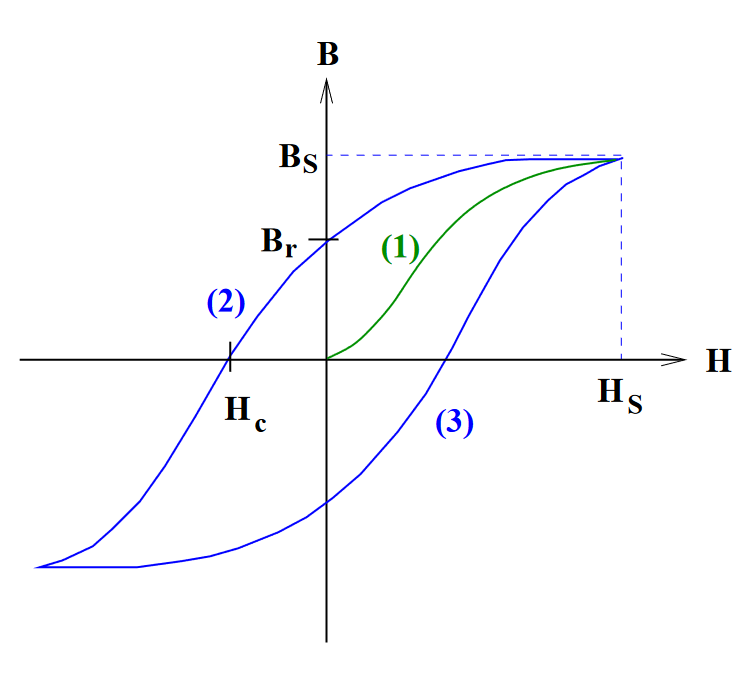
\includegraphics[height=5cm]{hysterese.png}
  \caption{Eine Hysteresekurve. \cite[S. 3]{sample}}
\end{figure}

In diesem Versuch wurde zur Berechnung der Theoriekurven oft die Gleichung
\begin{align}
B(x) = \frac{\mu_0 N I}{2l} \biggl( \frac{x}{\sqrt{R^{2} + x^{2}}} + \frac{l - x}{\sqrt{R^{2} + (l - x)^{2}}} \biggr) 
\end{align}
verwendet (Quelle: \cite[S. 5]{weltformel}), wobei $l$ die Länge, $N$ die Windungszahl und $R$ der 
Radius der Spule ist.